\documentclass{ieeeaccess}

\usepackage{cite}
\usepackage[T1]{fontenc}
\usepackage[utf8]{inputenc}
\usepackage{amsmath,amssymb,amsfonts,amsthm}
\usepackage{algorithm}
\usepackage{algpseudocode}
\usepackage{graphicx}
\usepackage{textcomp}
\usepackage{booktabs,array,tabularx}
\usepackage{calc}
\usepackage{etoolbox}
\usepackage{xcolor}
\usepackage{bm}
\usepackage{enumitem}

\makeatletter
% Fix algorithm caption alignment (prevent inter-word justification stretching in narrow IEEE columns)
\renewcommand\floatc@ruled[2]{{\raggedright\@fs@cfont #1\space\space #2\par}}

% Format algorithmic comments with clean alignment and hanging indent
\algrenewcomment[1]{\hfill\parbox[t]{0.52\linewidth}{\raggedright\hangindent=1em\hangafter=1\(\triangleright\)~#1}}

\AtBeginDocument{\DeclareMathVersion{bold}
\SetSymbolFont{operators}{bold}{T1}{times}{b}{n}
\SetSymbolFont{NewLetters}{bold}{T1}{times}{b}{it}
\SetMathAlphabet{\mathrm}{bold}{T1}{times}{b}{n}
\SetMathAlphabet{\mathit}{bold}{T1}{times}{b}{it}
\SetMathAlphabet{\mathbf}{bold}{T1}{times}{b}{n}
\SetMathAlphabet{\mathtt}{bold}{OT1}{pcr}{b}{n}
\SetSymbolFont{symbols}{bold}{OMS}{cmsy}{b}{n}
\renewcommand\boldmath{\@nomath\boldmath\mathversion{bold}}}
\makeatother

\def\BibTeX{{\rm B\kern-.05em{\sc i\kern-.025em b}\kern-.08em
    T\kern-.1667em\lower.7ex\hbox{E}\kern-.125emX}}

% ---------- theorem environments ----------
\theoremstyle{plain}
\newtheorem{theorem}{Theorem}[section]
\newtheorem{lemma}[theorem]{Lemma}
\newtheorem{proposition}{Proposition}[section]
\newtheorem{corollary}[theorem]{Corollary}
\theoremstyle{definition}
\newtheorem{definition}{Definition}[section]
\newtheorem{remark}{Remark}[section]

% ---------- math operators ----------
\DeclareMathOperator{\Runs}{Runs}
\DeclareMathOperator{\Inv}{Inv}
\DeclareMathOperator{\Rem}{Rem}
\DeclareMathOperator{\Exc}{Exc}
\DeclareMathOperator{\SortedSeq}{SortedSeq}
\newcommand{\tops}{\texttt{tops}}
\newcommand{\lastIdx}{\texttt{lastIdx}}

\setcounter{secnumdepth}{3}
\setlength{\emergencystretch}{3em}

\begin{document}

\history{Date of publication Month 00, 2026, date of current version Month 00, 2026.}
\doi{10.1109/ACCESS.2026.0000000}
\year{2026}
\vol{14}

\title{LadderSort: Adaptive Sorting via Interleaved Nondecreasing Subsequences}

\author{\uppercase{Malik M. H. Nayab}\authorrefmark{1},
\uppercase{Author 2}\authorrefmark{2}, AND
\uppercase{Author 3}\authorrefmark{3}}

\address[1]{COMSATS University Islamabad, Abbottabad Campus, Pakistan (e-mail: hamza.nayab48@gmail.com)}
\address[2]{COMSATS University Islamabad, Abbottabad Campus, Pakistan (e-mail: author2@cuiatd.edu.pk)}
\address[3]{COMSATS University Islamabad, Abbottabad Campus, Pakistan (e-mail: author3@cuiatd.edu.pk)}

\markboth
{Nayab \headeretal: LadderSort: Adaptive Sorting via Interleaved Nondecreasing Subsequences}
{Nayab \headeretal: LadderSort: Adaptive Sorting via Interleaved Nondecreasing Subsequences}

\corresp{Corresponding author: Malik M. H. Nayab (e-mail: hamza.nayab48@gmail.com).}

\begin{abstract}
Adaptive sorting algorithms take benefit of pre-existing structures in input to achieve performance better than $\Theta(N \log N)$. Traditional methods, like TimSort, estimate the presortedness measure based on contiguous runs. However, they prove to be less effective when input is based on interleaved sorted sequences. This paper presents LadderSort, a deterministic comparison-based sorting algorithm that adapts to $K$, the minimum number of nondecreasing subsequences covering the input, which equals both the offline optimum $K^*(A)$ and the length of the Longest strictly Decreasing Subsequence $\mathrm{LDS}(A)$. The algorithm operates in two phases: Phase~1 decomposes the input into $K$ nondecreasing ladders via a hinted greedy scan, and Phase~2 merges them using a $K$-adaptive strategy (galloping two-way merge for $K=2$, loser-tree $K$-way merge for $K>2$). LadderSort runs in $O(N\log(K+1))$ time and $O(N+K)$ auxiliary space, interpolating between linear time on sorted input and $O(N\log N)$ on adversarial input. Experiments on eight synthetic workloads and a real GH~Archive trace ($K=368$) confirm practical speedups over TimSort on small-$K$ interleaved inputs while preserving graceful degradation on adversarial inputs. We observe that LadderSort achieves faster execution time of up to 1.45 times over TimSort in wall-clock time on interleaved-stream workloads, particularly when $K \ll N$, while remaining competitive on random inputs, with a hybrid fallback variant ensuring graceful degradation on adversarial reverse-sorted inputs.
\end{abstract}

\begin{keywords}
adaptive sorting, presortedness measures, nondecreasing subsequences, multiway merge, loser tree, streaming data
\end{keywords}

\titlepgskip=-21pt

\maketitle

% ============================================================
\section{Introduction}
\label{sec:intro}
% ============================================================

\PARstart{S}{orting} is among the most fundamental primitives in algorithm design. It underpins database query processing, search-index construction, stream-join operators, analytics pipelines, and event-driven architectures.  Classical comparison-based algorithms achieve $\Theta(N\log N)$ worst-case time, which is information-theoretically optimal for arbitrary inputs.  However, data encountered in practice is rarely arbitrary.  In many modern systems, the input to a sort routine arrives not as a random permutation but as a {\em fan-in} of several locally ordered producer streams, such as event logs from distributed services, timestamped telemetry from a fleet of devices, social-media timelines merged for display, posting-list segments in search-index maintenance, venue-specific feeds in market-data processing, or partition outputs in data-pipeline fan-in stages.  Each producer emits a nondecreasing stream, and the aggregate sequence that reaches the sorting layer is a bursty, noncontiguous interleaving of those streams.  Such sequences carry substantial \emph{latent order} that a sufficiently adaptive algorithm can exploit to sort well below the $N\log N$ barrier.

To understand why run-adaptive sorting is not enough, consider the dominant family of adaptive sorting algorithms.  These algorithms, most notably TimSort \cite{Auger2018} and PowerSort \cite{MunroWild2018}, measure the exploitable order in a sequence $A$ by $\Runs(A)$, the number of maximal contiguous monotone blocks (``runs''). A contiguous run is only useful when consecutive sorted elements appear next to each other in memory. In the fan-in workloads, each producer stream is internally sorted, but records from different producers are interleaved in the aggregate buffer. The interleaving process fragments each stream into many short contiguous runs, such that every switch from one producer to another can start a new run. When context switches are frequent (e.g., the common case in bursty telemetry, round-robin feed merging, or consolidated market feeds), the run count satisfies $\Runs(A) = \Theta(N)$, even though, the sequence is an interleaving of only $K \ll N$ nondecreasing subsequences. Because the cost of run-adaptive algorithms is $O(N + N\log\Runs(A))$, they are forced into $\Theta(N\log N)$ behavior on precisely the workloads that carry the most exploitable structure. A sorting algorithm that measures cost by the number of interleaved sorted subsequences $K$ rather than by $\Runs(A)$ can sort in $O(N\log(K+1))$ time, equivalently $O(N\log K)$ for $K \ge 2$. To understand the noncontiguous order problem, suppose three devices produce timestamped records:
\[
  D_1: 3,\;7,\;8 \qquad
  D_2: 2,\;5     \qquad
  D_3: 4.
\]
An arrival buffer that interleaves these streams might contain $A = \langle 3,\;7,\;2,\;5,\;4,\;8 \rangle$. A run-adaptive algorithm performs several short contiguous runs ($\langle 3,7 \rangle$, then a drop to~2, and so on), yielding a high run count relative to $N$.  Yet the sequence is naturally explained as three nondecreasing subsequences (ladders) that can be recovered by a single left-to-right scan: $L_1 = (3,7,8)$, $L_2 = (2,5)$, $L_3 = (4)$. After the identification of ladders, the sorted output is produced by a 3-way merge mechanism. 

The aforementioned example highlights a major limitation of adaptive run algorithms. Although $A$ is generated from three initially sorted streams ($K=3$), run-based algorithms perceive a high degree of disorder because the sorted elements are not contiguous in memory. As a result, they fail to exploit the interleaved presortedness within the input and fall back to $O(N \log N)$ performance. This limitation motivates the need for a sorting algorithm that adapts to the interleaved presortedness of the structure instead of relying on $\Runs(A)$. To address this gap, this paper presents LadderSort, a comparison-based sorting algorithm that decomposes the input into small, nondecreasing ladders, which are then merged adaptively. The LadderSort algorithm operates in two phases:


\emph{Phase~1 (decomposition)}: In this phase, the input $A$ is traversed from left to right. Each key $x$ is appended to the leftmost ladder whose current tail is at most $x$. In case, no such ladder exists, a new ladder is created. The resulting decomposition produces $K$ nondecreasing ladders.

\emph{Phase~2 (adaptive merge)}: This phase merges the $K$ ladders using a strategy depending upon value of $K$: direct return for $K=1$, a galloping two-way merge for $K=2$, and a loser-tree $K$-way merge for $K > 2$.  The combined cost is $O(N\log(K+1))$ time, equivalently $O(N\log K)$ for $K \ge 2$, and $O(N+K)$ auxiliary space.

The parameter $K$ is not arbitrarily selected.  Under the algorithm's placement rule, the online ladder count $K_{\mathrm{LS}}(A)$ equals the offline optimum $K^*(A)$ (the minimum number of nondecreasing subsequences covering $A$), which in turn equals the length of the Longest strictly Decreasing Subsequence, i.e., $\mathrm{LDS}(A)$.  That is, $K_{\mathrm{LS}}(A) = K^*(A) = \mathrm{LDS}(A)$; the formal proof appears in Theorem~\ref{thm:greedy_optimal}.  LadderSort therefore performs best on inputs with small $K$ but many contiguous runs, particularly in interleaved-stream workloads where run-adaptive methods perform poorly.
The following is the summary of our contributions.

\begin{enumerate}

\item We propose LadderSort, a comparison-based sorting algorithm that exploits the presortedness measure $K$ and achieves
$O(N\log(K+1))$ running time using $O(N+K)$ auxiliary space.

\item Theoretical analysis of LadderSort is presented including correctness proofs, optimality of its ladder decomposition
($K_{\mathrm{LS}}(A)=K^*(A)=\mathrm{LDS}(A)$), and time, space, and average-case complexity analyses.

\item We show that the presortedness measure $K$ complements classical measures such as $\emph{Runs}$, capturing noncontiguous order that run-based measures cannot represent.

\item A hybrid variant of LadderSort is introduced that detects large-$K$ inputs and falls back to a conventional $O(N\log N)$ sorting algorithm to ensure robust worst-case performance.

\item Extensive experiments are conducted on synthetic and real-world datasets that depict that LadderSort is effective on small-$K$ interleaved-stream inputs, while it maintains graceful performance on adversarial workloads.

\end{enumerate}

The paper is organized as follows. The preliminaries and notations are discussed in Section~\ref{sec:prelim}. Literature review on adaptive sorting and presortedness measures is presented in Section~\ref{sec:related}. The LadderSort algorithm is explained in detail in Section~\ref{sec:algorithm}, including its two phases and the underlying placement rule. A theoretical analysis and proof of correctness, optimality, and time \& space complexity of LadderSort is presented in Section~\ref{sec:theory}. Performance evaluation results of LadderSort are presented in Section~\ref{sec:results} on synthetic and real-world datasets. Limitations and tradeoffs of the proposed algorithm are discussed in Section~\ref{sec:limits}. Finally, Section~\ref{sec:conclusion} concludes the paper and outlines directions for future research.


% ============================================================
\section{Background and Preliminaries}
\label{sec:prelim}
This section presents the notations and definitions used throughout the paper. The specific terminologies employed in the discussions of existing literature in Section 3 (Related Work~\ref{sec:related}) are also defined here. We assume a totally ordered domain $(\mathcal{D},\leq)$ from which a sequence of $N$ keys $A = \langle a_1, a_2, \ldots, a_N \rangle$ are drawn. We denote the set of integers from $1$ to $m$ as $\{1,2,\ldots,m\}$. The goal is to compute a nondecreasing permutation $S$ of $A$, where ``sorted'' means nondecreasing under the order $\leq$. In the rest of the paper, we use $\log$ to denote $\log_2$. Table~\ref{tab:notation} summarizes the primary mathematical notations.
 
\begin{table}[t]
\centering
\caption{Summary of mathematical notation.}
\label{tab:notation}
\begin{tabularx}{\linewidth}{@{}lX@{}}
\toprule
Notation & Description \\
\midrule
$A,N$ & Input sequence $A=\langle a_1,\ldots,a_N\rangle$ and its length $N$ \\
$K$ & Dynamic number of ladders (nondecreasing subsequences) produced by the algorithm \\
$K_{\mathrm{LS}}(A)$ & Formal function mapping $A$ to the ladder count produced by Phase~1 \\
$K^*(A)$ & Offline optimum: minimum number of nondecreasing subsequences covering $A$ \\
$\mathrm{LDS}(A)$ & Length of the longest strictly decreasing subsequence of $A$ \\
$\mathtt{tops}[1..K]$ & Contiguous array maintaining the tail (maximum) element of each active ladder \\
$\pi(x;\mathtt{tops})$ & Placement index: leftmost ladder $j$ such that $\mathtt{tops}[j] \leq x$ \\
$\oplus$ & Sequence concatenation operator (used in proofs) \\
$\prec$ & Total order for deterministic tie-breaking by ladder identifier during the merge \\
\bottomrule
\end{tabularx}
\end{table}
 
\begin{definition}[Classical presortedness measures]
\label{def:measures}
\begin{itemize}[leftmargin=*,itemsep=2pt,topsep=2pt]
\item[] $\mathrm{Runs}(A) :=$ number of maximal nondecreasing contiguous blocks in $A$.
\item[] $\mathrm{Inv}(A) := \bigl|\{(i,j) : i < j,\, a_i > a_j\}\bigr|$.
\item[] $\mathrm{Rem}(A) := N - $ length of longest nondecreasing subsequence of $A$.
\item[] $\mathrm{Exc}(A) :=$ minimum number of exchanges/transpositions to sort $A$.
\item[] $\mathrm{SortedSeq}(A) :=$ minimum number of nondecreasing subsequences whose union covers $A$.
\end{itemize}
\end{definition}
 
\begin{definition}[Ladder]
\label{def:ladder}
A \emph{ladder} is a finite sequence $L = \langle \ell_1, \ldots, \ell_m \rangle$ such that $\ell_1 \leq \ell_2 \leq \cdots \leq \ell_m$.
\end{definition}


\begin{definition}[Tail and tail array]
\label{def:tail}
For a nonempty ladder $L$, its \emph{tail} is defined as $\mathrm{tail}(L) := \ell_m$. 
Given an ordered collection of $K$ nonempty ladders $\mathcal{L} = (L_1, L_2, \ldots, L_K)$, 
the corresponding \emph{tail array} $\mathtt{tops}[1..K]$ is a contiguous array where 
$\mathtt{tops}[j] := \mathrm{tail}(L_j)$ for all $j \in [K]$. The collection $\mathcal{L}$ is 
said to satisfy the \emph{tail monotonicity property} if:
\[
  \mathtt{tops}[1] \geq \mathtt{tops}[2] \geq \cdots \geq \mathtt{tops}[K].
\]
\end{definition}


\begin{definition}[Placement index]
\label{def:placement}
For a key $x$ and a nonincreasing array $\mathtt{tops}[1..K]$, the \emph{placement index} is
\[
  \pi(x;\mathtt{tops}) := \min\bigl\{j \in [K] : \mathtt{tops}[j] \leq x\bigr\},
\]
taking $\pi(x;\mathtt{tops}) := K+1$ if no such $j$ exists.
\end{definition}
 

\begin{definition}[Greedy ladder count $K_{\mathrm{LS}}$]
\label{def:K}
Let $K_{\mathrm{LS}}(A)$ denote the total number of ladders constructed by sequentially processing 
the sequence $A$ from left to right under the online greedy placement rule specified in 
Definition~\ref{def:placement}. Alternatively, $K_{\mathrm{LS}}(A) = |\mathtt{tops}|$ upon 
consuming the final element of $A$. We reserve $K^*(A) := \mathrm{SortedSeq}(A)$ to denote the 
absolute offline optimal cover (Definition~\ref{def:measures}).
\end{definition}

\begin{definition}[Run-identifier tie-break]
\label{def:tiebreak}
During $K$-way merge, comparisons use the total order:
\[
  (x,j) \prec (y,\ell) \iff (x < y) \vee (x = y \wedge j < \ell),
\]
where $j, \ell \in [K]$ are ladder identifiers assigned in creation order. This makes the merge deterministic on duplicate keys. Note that the LadderSort is not globally stable.
\end{definition}


\begin{proposition}[Dilworth equality for sequences]
\label{prop:dilworth}
For any sequence $A$, let $K^*(A) := \SortedSeq(A)$ be the minimum number
of nondecreasing subsequences that cover $A$, and let $\mathrm{LDS}(A)$ be
the length of a longest strictly decreasing subsequence of $A$.  Then
\[ K^*(A) = \mathrm{LDS}(A). \]
\end{proposition}

The offline minimum $K^*(A)$ can be computed in $O(N\log N)$ time using standard patience-sorting routines \cite{Fredman1975,AldousDiaconis1999}. The following Theorem~\ref{thm:greedy_optimal} shows that the online greedy placement used in
Phase~1 (Section~\ref{sec:phase1}) achieves this offline optimum under our placement/tie convention.

\begin{theorem}[Optimality of the greedy ladder decomposition]
\label{thm:greedy_optimal}
For every input sequence $A$,
\[ K_{\mathrm{LS}}(A) = K^*(A) = \mathrm{LDS}(A). \]
\end{theorem}

Any strictly decreasing subsequence of length $r$ requires $r$ distinct nondecreasing subsequences in any cover, so $\mathrm{LDS}(A) \le K^*(A)$.
By Dilworth's Theorem (Proposition~\ref{prop:dilworth}), $K^*(A) = \mathrm{LDS}(A)$. Combining these inequalities:
\[ \mathrm{LDS}(A) \ge K_{\mathrm{LS}}(A), \quad K^*(A) \le K_{\mathrm{LS}}(A), \quad K^*(A) = \mathrm{LDS}(A). \]
Therefore, $K_{\mathrm{LS}}(A) = K^*(A) = \mathrm{LDS}(A)$.


% ============================================================
\section{Related Work}
\label{sec:related}
% ============================================================

In this section, we review the literature on adaptive sorting and presortedness measures, and compare LadderSort in the context of existing frameworks. We highlight the limitations of run-adaptive methods on interleaved-stream workloads and motivate the need for a measure that captures noncontiguous order.

\subsection{Existing Presortedness Frameworks}
\label{sec:measures}

Adaptive sorting theory formalizes algorithmic cost as a function of a \emph{measure of presortedness}: a mapping $m$ from a sequence $A$ of length $n$ to a non-negative integer satisfying standard monotonicity and normalization axioms~\cite{Mannila1985}. Mannila's foundational framework establishes that a measure $m$ is meaningful only if the execution cost of a sorting algorithm can be bounded as a function of both $n$ and $m(A)$, rather than $n$ alone~\cite{Mannila1985}. Notably, it is not required by the framework that an algorithm optimal with respect to $m_1$ be optimal with respect to $m_2$ if the two measures are not mutually bounded; different measures reflect different aspects of the input's structural properties.


Estivill-Castro and Wood~\cite{EstivillWood1992} study the presortedness measures of classical type, which includes the number of contiguous runs $\Runs(A)$, the number of inversions $\Inv(A)$, the removal distance $\Rem(A)$, and the exchange distance $\Exc(A)$ (see Section~\ref{sec:prelim}, Definition~\ref{def:measures}). These actions have been partially ranked according to their ability to discriminate. For example, for all sequences $A$; $\Inv(A) \ge \Runs(A) - 1$; therefore an algorithm optimal under $\Inv$ is automatically as adaptive as an algorithm optimal under $\Runs$ and the other way around is not true.

The measure $\SortedSeq(A)$, which is the number of minimal nondecreasing subsequences needed to cover $A$ is a unique entity in this hierarchy. A duality between covering and extremal sequences, between $\SortedSeq(A)$ and the longest strictly decreasing subsequence of $A$ is given by the celebrated Dilworth's Theorem~\cite{Dilworth1950}. LadderSort is designed specifically to address this structural property, with its $K$ parameter. In particular we prove in Theorem~\ref{thm:greedy_optimal} that the online ladder count equals $\SortedSeq(A) = \operatorname{LDS}(A)$.

Numerous existing works explore \emph{contiguous} monotone runs. An example is \emph{natural MergeSort} that analyzes existing runs and sequentially merges them~\cite{Knuth1998}. Its successor \emph{TimSort}~\cite{Auger2018} checks for ascending or descending runs, and utilizes binary insertion sort to enforce minimum run lengths. Using strict stack invariants, the \emph{TimSort} manages the merge sequence to guarantee an $O(N + N\log\Runs(A))$ time complexity. Alternatively, \emph{PowerSort}~\cite{MunroWild2018} constructs near optimal merge trees with minimal overhead, further refined by multiway extension~\cite{GellingNebel2023}.

In~\cite{Skiena1988}, the monotone subsequences are created by greedily extending lists from both ends. This yields a presortedness measure capturing a broader structural order than $\Runs(A)$. The classical hierarchy has tightly bound the number of \emph{encroaching lists} between $\SortedSeq(A)$ and $\Runs(A)$. Similarly, the classical online greedy procedure, \emph{patience sorting}~\cite{AldousDiaconis1999} has pile count corresponding directly to extremal subsequence lengths. It tracks the longest increasing subsequence $\operatorname{LIS}(A)$ or decreasing subsequence $\operatorname{LDS}(A)$ depending upon specific convention used for tie-breaking convention.

The general purpose algorithms (Introsort~\cite{Musser1997, CLRS2022}, BlockQuicksort~\cite{Edelkamp2016} and Smoothsort~\cite{Dijkstra1981}) have $O(N \log N)$ worst cases, but they are not aware of the structure of the input, and they do not take advantage of the presortedness. Tournament-like structures work very well with input sequences of multiway ordered streams. The \emph{loser-tree} variant is also of major importance in $K$-way external-memory merging pipelines~\cite{Knuth1998}. Initially, a loser tree with $K$ leaves can be initialized in $O(K)$ time; each extract-minimum-and-advance step can be performed in $O(\log K)$ time. The loser of each match is stored at the internal nodes, which reduces the number of memory accesses yielding $\lceil \log K \rceil$ for each step as opposed to $2\lceil \log K\rceil$ for a typical winner tree. Hence, this architecture is commonly used in external sorting scenarios~\cite{Aggarwal1988,Polyntsov2022} for managing stream of large volumes of data.


\subsection{The Interleaving Gap}
\label{sec:interleaving_gap}

In all the run-adaptive methods which have been surveyed above (TimSort, PowerSort, AdaptiveShiversSort, and natural mergesort), the cost is a function of $\Runs(A)$ representing the number of \emph{contiguous} maximal monotone blocks. Such measure is suitable for inputs arriving as a few long sorted segments (e.g., log rotations, append-dominated tables, or nearly sorted files), but it is unable to tell that the input is \emph{noncontiguously} ordered. Considering $K$ internally sorted producer streams that are interleaved and multiplexed into a single buffer in arrival order, with each producer contributing approximately $N/K$ elements, every context switch from one producer to another may break a contiguous run. Usually, a sequence is an interleaving of only $K$ nondecreasing subsequences, however, when the number of context switches is high (the usual situation for bursty telemetry, round robin feed merging or consolidated feed from the financial markets), the number of contiguous runs goes to $\Runs(A) = \Theta(N)$. In such case, run adaptive sorts exhibit worst-case behavior on the workloads that have the most exploitable structure.

The above-mentioned performance gap stems from a fundamental mismatch between the actual structural parameter of the input sequence and the measure used by the algorithm. The appropriate parameter to exploit is the global optimal cover, $K = \SortedSeq(A)$, representing the minimum number of nondecreasing subsequences spanning $A$. In the interleaved-stream scenario, $K \ll N$ and $K \ll \Runs(A)$; consequently, an algorithm that adapts to $K$ instead of $\Runs(A)$ can achieve a time complexity of $O(N \log (K + 1))$. For any $K \ge 2$, this collapses to an optimal $O(N \log K)$ bound, offering massive performance gains over the oblivious $O(N \log N)$ worst-case bound.

Encroaching lists proposed in~\cite{Skiena1988} partially mitigate the inability of run-adaptive sorting algorithms to recognize noncontiguous order structure. They primarily function as online partitioning mechanism to perform recognition of noncontiguous subsequence structures, but lack a deterministic merge policy that guarantees a strict $O(N \log (K + 1))$ execution bound. Alternatively, Aldous \emph{et al.}~\cite{AldousDiaconis1999} proposed patience sorting that performs an online sequence partition optimal count, but it lacked an integrated $K$-adaptive merge phase to synthesize the sorted output. Therefore, it remains an open challenge to bridge the gap between online noncontiguous partitioning and optimal multiway merging.
 
To consider the proposed $K$ in the context of existing presortedness measures, we assume that $K_{\mathrm{LS}}(A)$ represents the number of the ladders created by the online greedy placement rule of LadderSort, i.e., Definition~\ref{def:placement}. This ladder count not only equals the  offline optimal decomposition $K^*(A)$, but also equals the length of longest decreasing subsequence:
%
\[
K_{\mathrm{LS}}(A)=K^*(A)=\mathrm{LDS}(A)\le \Runs(A).
\]
%

The above inequality indicates that instead of capturing only the contiguous runs, these ladders also capture the globally ordered subsequences. For instance, if the input is formed by interleaving $K_0$ nondecreasing subsequences, then we have $K_{\mathrm{LS}}(A)\le K_0$. The equality holds when a decreasing subsequence of length $K_0$ exists in the interleaving. Consequently, $\Runs(A)$ can be $\Theta(N)$, keeping the ladder decomposition optimal. This shows that $K$ can capture the different forms of input order  that are not detected by run-based measures.

The proposed measure is also related to inversion-based presortedness. For certain families of input sequences, $\Inv(A)\ge\binom{K}{2}$, implying the asymptotic bound $K=O(\sqrt{\Inv(A)})$. Thus, although inversion count and ladder count are related, they characterize different aspects of existing order.


\subsection{Offline Sequence Decomposition}
\label{sec:dilworth}

Dilworth's theorem gives a clean characterization of optimal sequence decomposition. The minimum number of nondecreasing subsequences needed to cover a sequence equals the length of its longest strictly decreasing subsequence~\cite{Dilworth1950}. In the current context, this implies that:
\[
K^*(A) = \mathrm{LDS}(A),
\]
where $K^*(A)$ denotes the optimal offline ladder count which can be computed in $O(N\log N)$ time using  patience-sorting-based routines~\cite{Fredman1975,AldousDiaconis1999}. Such methods treat decomposition as an offline objective or as a presortedness measure, and not as the preliminary stage of a sorting algorithm.

In LadderSort, the ladders are constructed through an online greedy placement algorithm during input parsing, and merged to generate the sorted output. As will be shown in Section~\ref{sec:theory}, this online decomposition process yields the optimal count consistent with Dilworth's theorem, while adhering to a complete $K$-adaptive sorting framework.

%-----------------------------------------------------------------------
% ============================================================
\section{The LadderSort Algorithm}
\label{sec:algorithm}
% ============================================================
We present the LadderSort algorithm including its both phases and basic placement rule. The algorithm is designed to take benefit of presortedness measure $K$, achieving optimal performance on interleaved-stream workloads, and show graceful performance degradation on adversarial inputs. Moreover, the LadderSort utilizes the three-way integrated approach to reduce the interleaving gap discussed in Section~\ref{sec:interleaving_gap}. 

\subsection{Overview}

LadderSort operates in two distinct phases (conceptually illustrated in Figure~\ref{fig:overview}):

\begin{figure*}[t]
\centering
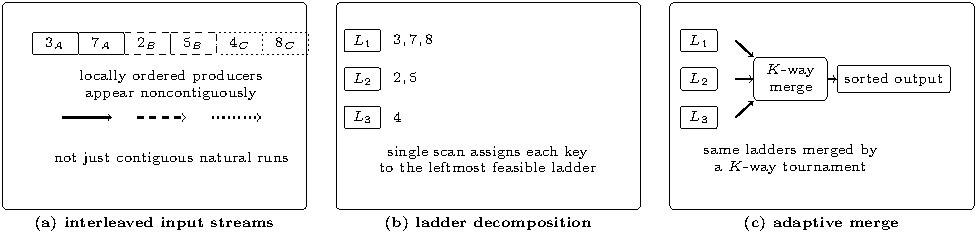
\includegraphics[width=0.92\linewidth]{media/overview_diagram.pdf}
\caption{LadderSort targets input profiles that present as interleavings of locally ordered data streams. Phase~1 decomposes the sequence into nondecreasing ladders via an online leftmost-feasible placement rule; in this trace, $L_1=(3,7,8)$, $L_2=(2,5)$, and $L_3=(4)$. Phase~2 merges these subsystems adaptively, guaranteeing an optimal overall complexity of $O(N \log (K + 1))$.}
\label{fig:overview}
\end{figure*}


\subsection{Phase 1: Sequential Decomposition}
\label{sec:phase1}

Phase~1 decomposes the input sequence $A$ into an organized collection of non-decreasing ladders, represented as $\mathcal{L} = (L_1, L_2, \ldots, L_K)$. The input is scanned from left to right and using an online greedy placement rule, places the incoming key to left most feasible ladder (using Definition~\ref{def:placement}). Moreover, it keeps the tail array $\tops$ into a strictly decreasing order (Definition~\ref{def:tail}). The aforementioned strategy limits the search problem to find the smallest index $j$ where $\tops[j] \le x$.

The proposed design is inspired by the classical patience-sorting technique~\cite{AldousDiaconis1999}. By combining sorted tail vector with monotonic search predicate, the online rule absolutely achieves $K_{\mathrm{LS}}(A) = \SortedSeq(A) = \mathrm{LDS}(A)$ ladders (Theorem~\ref{thm:greedy_optimal}). In previous works, such decompositions are considered as static offline measures. On the contrary, the LadderSort utilizes this feature as a stateful first stage prior to optimal multi-way merge.

Algorithm~\ref{alg:laddersort} provides an overview of the whole process. All routing decisions are handed over to \textsc{HintedLowerBound} (Algorithm~\ref{alg:hinted}) by the main routine. This subroutine utilizes three-phase locality-aware search to find insertion index in worst case $O(\log K)$. 

\subsubsection{Sequential Decomposition Mechanics}

The main decomposition loop processes the input in a single pass and tracks active tail of each ladder in $\tops$ vector. The algorithm reduces the lookup overhead for those consecutive elements that arrive from the same stream producer. It accomplishes this by caching the latest modified insertion position ($\lastIdx$) and passing it to the search subroutine. This stateful tracking measure effectively maintains a communication between pipeline's macroscopic fan-in structure and microscopic element placement logic, and ensures to take full advantage of temporal locality.

\begin{algorithm}[t]
\caption{\textsc{LadderSort}$(A)$}
\label{alg:laddersort}
\begin{algorithmic}[1]
\Require Input sequence $A = \langle a_1, \dots, a_N \rangle$
\Ensure Sorted sequence $S$
\State Initialize empty ladder list $(L_1,\dots,L_K)$, $K \gets 0$
\State Initialize empty array $\tops$
\State $\lastIdx \gets 1$
\For{$i = 1$ to $N$}
    \State $x \gets a_i$
    \State $j \gets \textsc{HintedLowerBound}(\tops, x, \lastIdx)$
    \If{$j = K + 1$}
        \State $K \gets K + 1$;\quad $L_K \gets \langle x \rangle$;\quad $\tops[K] \gets x$
    \Else
        \State Append $x$ to $L_j$;\quad $\tops[j] \gets x$
    \EndIf
    \State $\lastIdx \gets j$
\EndFor
\State \Return $\textsc{MergeByK}(L_1, \dots, L_K)$
\end{algorithmic}
\end{algorithm}

\subsubsection{Stateful Hinting and Memory Layout}
The placement search over the tail array is accelerated via a stateful three-stage procedure designed to exploit the temporal patterns of interleaved fan-in streams:
\begin{enumerate}
  
\item \textbf{Stage 1 (Local Probe):} It checks whether the current element can be appended with the ladder that was updated in the previous iteration ($j = \lastIdx$). This helps in achieving $O(1)$ processing when consecutive tokens are arriving from the same producer.

\item \textbf{Stage 2 (Exponential Gallop):} If the local probe fails, this stage passes a search interval by exponentially doubling the stride parameter at the right of hint parameter till a valid boundary or end of array is encountered.

\item \textbf{Stage 3 (Binary Search):} 

This stage finds the exact insertion position in the bounded interval and guarantees a strict worst-case cost $O(\log K)$ for each element. It helps to maintain $O(1)$ performance in normal high-locality workloads.

\end{enumerate}

\begin{algorithm}[t]
\caption{\textsc{Hinted\-Lower\-Bound}$(\tops[1..K], x, \lastIdx)$}
\label{alg:hinted}
\begin{algorithmic}[1]
\Require Nonincreasing tail vector $\tops[1..K]$, target key $x$, historical hint $\lastIdx \in [1, K]$
\Ensure First index $j \in [K]$ satisfying $\tops[j] \le x$, or $K+1$ if no such position exists
\If{$K = 0$}
    \State \Return $1$ \Comment{First element initializes the primary ladder}
\EndIf
\Statex
\State \textbf{Stage 1: Local Probe}
\If{$\tops[\lastIdx] \le x$}
    \State \Return $\lastIdx$ \Comment{Element appends to the immediate prior ladder}
\EndIf
\Statex
\State \textbf{Stage 2: Exponential Gallop}
\State $s \gets 1$
\While{$\lastIdx + s \le K$ and $\tops[\lastIdx + s] > x$}
    \State $s \gets 2 \cdot s$
\EndWhile
\State $\mathit{lo} \gets \lastIdx + \lfloor s/2 \rfloor$
\State $\mathit{hi} \gets \min(K, \lastIdx + s)$
\Statex
\State \textbf{Stage 3: Binary Search}
\State $j \gets K + 1$
\While{$\mathit{lo} \le \mathit{hi}$}
    \State $\mathit{mid} \gets \mathit{lo} + \lfloor (\mathit{hi} - \mathit{lo}) / 2 \rfloor$
    \If{$\tops[\mathit{mid}] \le x$}
        \State $j \gets \mathit{mid}$;\quad $\mathit{hi} \gets \mathit{mid} - 1$ \Comment{Search left for smaller valid index}
    \Else
        \State $\mathit{lo} \gets \mathit{mid} + 1$
    \EndIf
\EndWhile
\State \Return $j$
\end{algorithmic}
\end{algorithm}

The array $\tops[1..K]$ is physically allocated as a contiguous memory vector. For practical workload dimensions where $K \ll \Runs(A)$, this structure remains highly compact and cache-resident, making the localized search sweeps exceptionally cache-friendly. We purposely refrain from making specific assertions regarding exact hardware performance metrics (such as target cache lines, translation lookaside buffer hit rates, or speculative branch behaviors) as these dynamics are heavily dependent on target execution environments and architectural specifications.


\subsection{Phase 2: Adaptive Merge Architecture}
\label{sec:phase2}
Phase~2 converts the sorted nondecreasing ladders $\mathcal{L}$ into a single globally ordered output sequence $S$. Execution paths are selected dynamically based on actual ladder count $K$. A direct return is made for $K=1$, optimized galloping two-way merge (Algorithm~\ref{alg:gallop}) is performed for $K=2$, and for $K > 2$, the deterministic $K$-way loser-tree merge (Algorithm~\ref{alg:loser}) is utilized. When multi-way streams  ($K > 2$) are processed, then for each extracted element, the tournament-style loser tree performs an upward update path with a maximum of $\lceil \log K \rceil$ comparisons. The ties are deterministically broken using ladder identifier (Definition~\ref{def:tiebreak}) that results in reproducible output. The combined complexity of sequence decomposition phase (Phase 1) and adaptive merging (Phase 2) comes up to $O(N \log (K + 1))$, while auxiliary workspace requires $O(N + K)$.

\subsubsection{Adaptive Flow Control}

Multi-path control logic plays an important role as a low-overhead algorithmic guardrail. It is designed to counter execution penalties that occur during processing of those inputs whose structures are highly localized. When $K=1$, the system completely bypasses the merging framework and returns the single pre-sorted ladder. This guarantees a strict $O(N)$ linear-time execution on pre-ordered inputs. When $K=2$, the execution branches into a specialized two-way galloping loop. This reduces the structural overhead in initializing and updating the internal tournament structure. Generalized multi-way tournament tree is reserved for those situations where $K > 2$. In this way, the initialization cost and tree traversal penalties occur only when dataset's fan-in complexity necessitates them. 


\begin{algorithm}[t]
\caption{\textsc{MergeByK}$(L_1, \dots, L_K)$}
\label{alg:mergebyk}
\begin{algorithmic}[1]
\Require Collection of nondecreasing ladders $\mathcal{L} = (L_1, \dots, L_K)$
\Ensure Globally sorted sequence $S$
\If{$K = 0$} 
    \State \Return $\langle\rangle$
\EndIf
\If{$K = 1$} 
    \State \Return $L_1$
\EndIf
\If{$K = 2$} 
    \State \Return $\textsc{TwoWayGalloping}(L_1, L_2)$
\EndIf
\State \Return $\textsc{KWayLoserTree}(L_1, \dots, L_K)$
\end{algorithmic}
\end{algorithm}

\subsubsection{Galloping Merge Strategy}

To take benefit of long-range monotonic runs in the generated ladders, galloping merge loop is utilized only for $K=2$. Instead of comparing with each element during merge procedure, the algorithm uses binary search following exponential search so that a specific contiguous block can be recognized which can be safely emitted~\cite{Ghasemi2024}. When the two ladders alternate in short turns, this becomes nearly similar to element-by-element comparisons. If a ladder dominates on some larger range, then block of length $r$ can be identified in $O(\log r)$ comparisons, and then it is emitted with a single pointer update.

\begin{algorithm}[t]
\caption{\textsc{TwoWayGalloping}$(L_1, L_2)$}
\label{alg:gallop}
\begin{algorithmic}[1]
\Require Sorted input ladders $L_1$ and $L_2$
\Ensure Sequentially merged sorted output sequence $S$
\State $p \gets 1$;\quad $q \gets 1$;\quad $S \gets \langle\rangle$

\While{$p \le |L_1|$ \textbf{and} $q \le |L_2|$}
    \If{$L_1[p] \le L_2[q]$}
        \State $s \gets 1$ \Comment{Exponential gallop rightward in $L_1$}
        \While{$p + s \le |L_1|$ and $L_1[p + s] \le L_2[q]$}
            \State $s \gets 2 \cdot s$
        \EndWhile
        \State $\mathit{lo} \gets p + \lfloor s/2 \rfloor$;\quad $\mathit{hi} \gets \min(|L_1|, p + s)$
        \State $r \gets \mathit{lo}$ \Comment{Binary search for the upper bound prefix}
        \While{$\mathit{lo} \le \mathit{hi}$}
            \State $\mathit{mid} \gets \mathit{lo} + \lfloor (\mathit{hi} - \mathit{lo}) / 2 \rfloor$
            \If{$L_1[\mathit{mid}] \le L_2[q]$}
                \State $r \gets \mathit{mid}$;\quad $\mathit{lo} \gets \mathit{mid} + 1$
            \Else
                \State $\mathit{hi} \gets \mathit{mid} - 1$
            \EndIf
        \EndWhile
        \State Append prefix $L_1[p..r]$ to $S$;\quad $p \gets r + 1$
    \Else
        \State $s \gets 1$ \Comment{Analogous exponential gallop rightward in $L_2$}
        \While{$q + s \le |L_2|$ \textbf{and} $L_2[q + s] < L_1[p]$}
            \State $s \gets 2 \cdot s$
        \EndWhile
        \State $\mathit{lo} \gets q + \lfloor s/2 \rfloor$;\quad $\mathit{hi} \gets \min(|L_2|, q + s)$
        \State $r \gets \mathit{lo}$
        \While{$\mathit{lo} \le \mathit{hi}$}
            \State $\mathit{mid} \gets \mathit{lo} + \lfloor (\mathit{hi} - \mathit{lo}) / 2 \rfloor$
            \If{$L_2[\mathit{mid}] < L_1[p]$}
                \State $r \gets \mathit{mid}$;\quad $\mathit{lo} \gets \mathit{mid} + 1$
            \Else
                \State $\mathit{hi} \gets \mathit{mid} - 1$
            \EndIf
        \EndWhile
        \State Append prefix $L_2[q..r]$ to $S$;\quad $q \gets r + 1$
    \EndIf
\EndWhile
\State Append any remaining elements from $L_1[p..|L_1|]$ or $L_2[q..|L_2|]$ directly to $S$
\State \Return $S$
\end{algorithmic}
\end{algorithm}

\subsubsection{Loser-tree Memory Layout}
For the general case ($K>2$), the loser tree is represented as an implicit binary tree stored in a flat array of $K$ integer entries, following the standard heap-array organization~\cite{Knuth1998}. Entry $T[0]$ stores the current overall winner, while the remaining $K-1$ entries record the losers of the internal tournament matches. An auxiliary array of $K$ head pointers maintains the current front element of each ladder. After each output element is produced, only the path from the corresponding leaf to the root is replayed to restore the tournament, requiring a single upward traversal of at most $\lceil\log K\rceil$ internal nodes. This compact representation requires $O(K)$ auxiliary memory and is well suited to efficient tournament updates while avoiding unnecessary pointer-based structures.


\begin{algorithm}[t]
\caption{\textsc{KWayLoserTree}$(L_1, \dots, L_K)$}
\label{alg:loser}
\begin{algorithmic}[1]
\Require $K$ nondecreasing sequences; comparison order $\prec$ (Definition~\ref{def:tiebreak})
\Ensure Globally sorted merge $S$
\State Allocate internal loser-tree array $T[0..K-1]$ (node 0 = overall winner)
\State Initialize: for $j = 1$ to $K$, $\mathit{head}[j] \gets$ first element of $L_j$
\State Run $K-1$ comparisons to build initial tournament; record losers at each internal node
\While{any sequence non-empty}
    \State $j^* \gets T[0]$ \Comment{index of overall winner (minimum)}
    \State Emit $\mathit{head}[j^*]$
    \State Advance $L_{j^*}$ by one element; update $\mathit{head}[j^*]$ (or $+\infty$ if exhausted)
    \State Walk path from leaf $j^*$ to root, comparing with stored losers and updating $T$
    \Comment{$\lceil \log K \rceil$ comparisons; each node stores loser, so path = single upward pass}
\EndWhile
\State \Return $S$
\end{algorithmic}
\end{algorithm}




 
% ============================================================
\section{Theoretical Analysis}
\label{sec:theory}
% ============================================================
In this section, we analyze the correctness and complexity of LadderSort.  We prove that the online greedy placement rule produces an optimal decomposition into $K$ nondecreasing ladders, and that the subsequent merge phase produces a globally sorted output.  We then analyze the time and space complexity of both phases, showing that the overall algorithm runs in $O(N \log (K + 1))$ time with $O(N + K)$ auxiliary space.

\subsection{Correctness}
\label{sec:correctness}

\begin{lemma}[Each ladder remains sorted]
\label{lem:ladder_sorted}
After processing any prefix $\langle a_1, \dots, a_t \rangle$ in Phase~1,
every ladder $L_j$ is nondecreasing.
\end{lemma}

\begin{proof}
Induction on $t$.  Base case $t=1$: $L_1 = \langle a_1 \rangle$ is
trivially nondecreasing.  Inductive step: assume all ladders are
nondecreasing after processing $a_1, \dots, a_{t-1}$.  At step $t$,
$x = a_t$ is assigned to ladder $L_j$ where $j = \pi(x;\tops)$.  If
$j = K+1$, a new singleton ladder $\langle x \rangle$ is created, which
is sorted.  Otherwise, $j$ is the first index with $\tops[j] \le x$, so
$\tops[j] = \mathrm{tail}(L_j) \le x$; appending $x$ to $L_j$ preserves
the nondecreasing property.  All other ladders are unchanged.
\end{proof}

\begin{lemma}[Strict tail invariant]
\label{lem:tops_nonincreasing}
After each insertion step of Phase~1 the tail array satisfies the strict
inequality
\[ \tops[1] > \tops[2] > \cdots > \tops[K]. \]
In particular the array is nonincreasing and, in fact, strictly decreasing
at all times.
\end{lemma}

\begin{proof}
We prove by induction on the number of processed elements that
$\tops[1] > \tops[2] > \cdots > \tops[K]$ is maintained.

\emph{Base case.} After the first insertion, $K=1$ and the invariant is vacuously true.

\emph{Inductive step.} Assume the invariant $\tops[1] > \tops[2] > \cdots > \tops[K]$ holds
before inserting element $x$. Let $j = \pi(x; \tops)$ be the first feasible index.

\textit{Case $j = K+1$ (new ladder).}
Then $x < \tops[p]$ for all $p \in [1..K]$, so $x < \tops[K]$.
We set $\tops[K+1] := x$. By the induction hypothesis, the old sequence
$\tops[1] > \cdots > \tops[K]$ is strictly decreasing. Since $x < \tops[K]$,
the new sequence $\tops[1] > \cdots > \tops[K] > \tops[K+1]$ is also strictly decreasing.

\textit{Case $j \le K$ (update existing ladder).}
We update $\tops[j] := x$.

For $p < j$: by definition of the first-feasible rule, $\tops[p] > x$. These values are unchanged.

For $p = j$: the new value is $x$.

For $p > j$: the values $\tops[p]$ are unchanged. By the induction hypothesis,
$\tops[j] > \tops[j+1]$ held before the update. Since the old $\tops[j] \le x$
(by feasibility), we have $\tops[j+1] < \tops[j] \le x$, thus $\tops[j+1] < x$.
After the update, the new value at position $j$ is $x$ and at position $j+1$ is $\tops[j+1]$,
so $x > \tops[j+1]$.

Boundary cases: If $j=1$, there are no positions $p<1$. If $j=K$, there are no positions $p>K$.
Both cases are covered by the logic above.

Therefore, the updated sequence $\tops[1] > \cdots > \tops[K]$ remains strictly decreasing.
\end{proof}

\begin{lemma}[Merge outputs a globally sorted list]
\label{lem:merge_sorted}
Assume $L_1, \dots, L_K$ are nondecreasing.  Then
$\textsc{MergeByK}(L_1, \dots, L_K)$ outputs a nondecreasing sequence $S$
that is a permutation of the multiset union $\bigcup_{j=1}^K L_j$.
\end{lemma}

\begin{proof}
\emph{$K \in \{0,1\}$:} Trivial.

\emph{$K = 2$:} \textsc{TwoWayGalloping} is a standard merge
(accelerated by galloping, which only extends contiguous blocks that are
provably $\le$ the opposing head).  Galloping does not alter correctness,
only the number of comparisons.  The result is a sorted permutation of
$L_1 \cup L_2$.

\emph{$K > 2$:} \textsc{KWayLoserTree} maintains one current head per
ladder and repeatedly outputs the minimum head under $\prec$
(Definition~\ref{def:tiebreak}).  Since each $L_j$ is nondecreasing,
advancing any pointer never decreases that ladder's head.  At each step,
the loser tree correctly identifies the global minimum head (by the
standard correctness argument for tournament trees \cite{Knuth1998}),
outputs it, advances the corresponding ladder, and restores the
tournament in $O(\log K)$ time.  Because $\prec$ is a total order
refining $\le$, the output sequence is nondecreasing in key order.
Every element is output exactly once, so $S$ is a permutation of the
union.
\end{proof}

\begin{theorem}[Correctness of LadderSort]
\label{thm:correctness}
For any input $A = \langle a_1, \dots, a_N \rangle$ over a totally
ordered domain, \textsc{LadderSort}$(A)$ outputs a sequence $S$ that is
(i) a permutation of $A$ and (ii) nondecreasing under $\le$.
\end{theorem}

\begin{proof}
By Lemma~\ref{lem:ladder_sorted}, each $L_j$ produced in Phase~1 is
nondecreasing.  Every element $a_i$ is appended to exactly one ladder
(or starts a new one), so the multiset union of the ladders equals $A$.
Lemma~\ref{lem:tops_nonincreasing} ensures the tail-array invariant is
maintained throughout, guaranteeing that the placement predicate is
applied correctly.  By Lemma~\ref{lem:merge_sorted}, Phase~2 outputs a nondecreasing permutation of the union, which equals a nondecreasing permutation of~$A$. The overall implementation control flow of the decomposition and merge phases is illustrated in the flowchart of Figure~\ref{fig:laddersort-flowchart}.
\end{proof}

\begin{figure}[t]
\centering
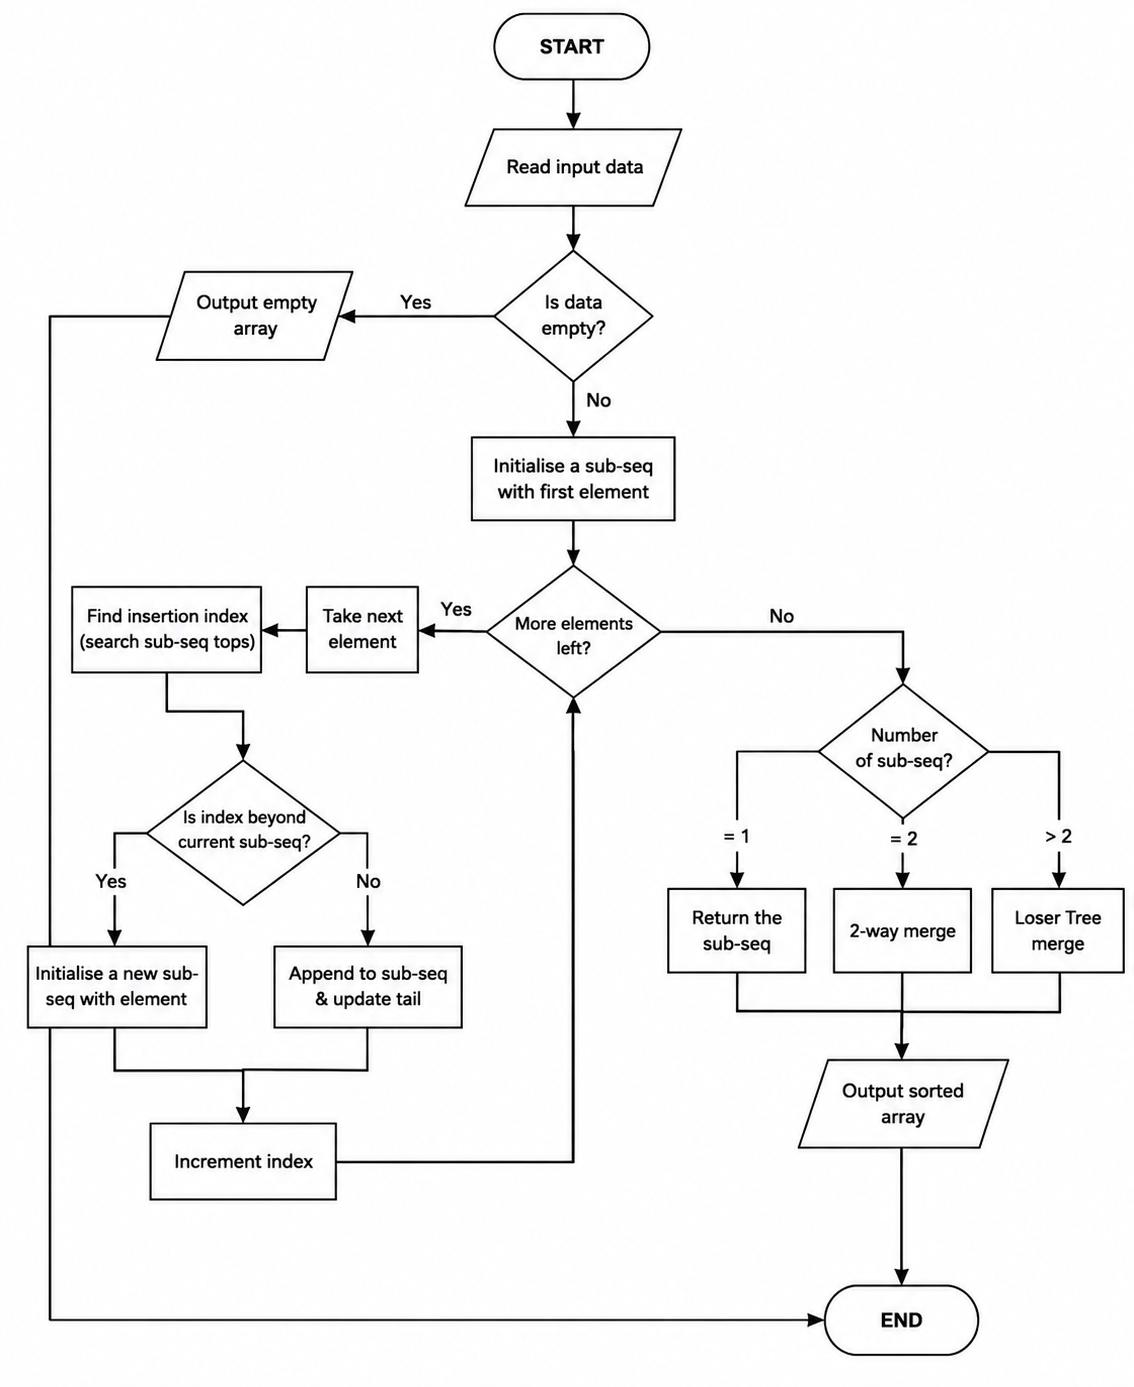
\includegraphics[width=0.82\linewidth]{media/updated_flow.png}
\caption{Implementation flowchart of LadderSort. The diagram summarises the
  decomposition and merge control flow, complementing the conceptual
  overview in Figure~\ref{fig:overview}.}
\label{fig:laddersort-flowchart}
\end{figure}

\subsection{Time Complexity}
\label{sec:timecomplexity}

\begin{lemma}[Time complexity]
\label{lem:complexity}
\textsc{LadderSort} runs in $O(N\log(K+1))$ time. More precisely, the algorithm is linear for $K=1$ and runs in $O(N\log K)$ for $K \ge 2$.
\end{lemma}

\begin{proof}
\emph{Phase~1.}  Each of the $N$ elements requires one call to
\textsc{HintedLowerBound}.  Stage~1 (local probe) costs $O(1)$.
Stage~2 (exponential gallop) doubles the stride until it reaches a
feasible index or overshoots $K$; the number of doublings is
$O(\log K)$.  Stage~3 (binary search within the bounded interval of
length at most $2s \le 2K$) costs $O(\log K)$.  Hence each placement
costs $O(\log K)$ in the worst case, giving Phase~1 cost $O(N \log(K+1))$.

\emph{Phase~2.}  For $K = 1$, the merge is $O(N)$ (return the single ladder).
For $K = 2$, the merge is $O(N)$ (binary merge overhead).  For $K > 2$, \textsc{KWayLoserTree} builds in $O(K)$ time
and performs $N$ extract-minimum steps each costing $O(\log K)$, for
total $O(K + N\log K) = O(N\log K)$ (since $K \le N$).

Combining both phases: $T(N, K) = O(N\log(K+1))$.
\end{proof}

For high-$K$ inputs (where $K$ approaches $N$ and LadderSort's overhead exceeds that of a non-adaptive sort), a hybrid variant monitors $K$ during decomposition and falls back to a standard $O(N\log N)$ sort when $K$
exceeds a configurable threshold.  This preserves LadderSort's small-$K$ path without penalizing adversarial inputs.


\begin{remark}
The bound $T(N,K)=O(N\log(K+1))$ interpolates correctly: $T(N,1)=O(N)$ and $T(N,N)=O(N\log N)$.  For $K = N^{o(1)}$ (e.g.\ $K = O((\log N)^c)$),
the cost is $o(N \log N)$.
\end{remark}


\subsection{Average-Case Analysis}
\label{sec:avgcase}

For a \emph{uniformly random permutation} of $N$ distinct keys, we bound the
expected value of $K$ produced by the LadderSort placement rule.

\begin{proposition}[Expected $K$ under uniform random permutation]
\label{prop:avgcase}
Let $A$ be a uniformly random permutation of $\{1, \dots, N\}$.  The
expected number of ladders produced by \textsc{LadderSort} satisfies
\[
  \mathbb{E}[K] = \Theta(\sqrt{N}).
\]
\end{proposition}

\begin{proof}
By Theorem~\ref{thm:greedy_optimal} we have $K=K_{\mathrm{LS}}(A)=\mathrm{LDS}(A)$.
Classical results on longest increasing/decreasing subsequences in random
permutations (Vershik--Kerov \cite{VershikKerov1977},
Logan--Shepp \cite{LoganShepp1977}, and the survey by
Aldous--Diaconis \cite{AldousDiaconis1999}) imply that the expected length
of the longest decreasing subsequence of a uniform random permutation of
$[N]$ is $\Theta(\sqrt{N})$ (in fact $2\sqrt{N}+o(\sqrt{N})$).  Hence
$\mathbb{E}[K]=\Theta(\sqrt{N})$.
\end{proof}

\begin{corollary}[Average-case complexity]
\label{cor:avgcase}
For a uniformly random permutation of $N$ distinct keys, classical results
on longest decreasing subsequences imply $\mathbb{E}[K]=\Theta(\sqrt{N})$.
Therefore, under the equality $K=\mathrm{LDS}(A)$ established above,
\[ \mathbb{E}[T(N,K)] = O\bigl(N\mathbb{E}[\log K]\bigr) = O(N\log\sqrt{N}) = O\bigl(N\tfrac{1}{2}\log N\bigr).
\]
The constant $\tfrac{1}{2}$ arises from the $\sqrt{N}$ scaling of $K$; one
may obtain the sharper $2\sqrt{N}+o(\sqrt{N})$ asymptotic for $\mathbb{E}[K]$
from Vershik--Kerov and Logan--Shepp via Aldous--Diaconis \cite{VershikKerov1977,LoganShepp1977,AldousDiaconis1999}.
\end{corollary}


This asymptotic is consistent with the empirical comparison counts in
Section~\ref{sec:results}: on random inputs LadderSort behaves like an
algorithm whose logarithmic factor is about $\tfrac{1}{2}\log N$ on average.

\subsection{A lower bound for the K-interleaving promise}
\label{sec:lowerbound}

To contextualise LadderSort's $O(N\log(K+1))$ bound, we give a simple
information-theoretic lower bound for the class of inputs that are
interleavings of $K$ labeled sorted subsequences.

\begin{proposition}[Worst-case comparison lower bound under $K$-interleaving]
\label{prop:lowerbound}
Consider the set of sequences formed by interleaving $K$ labeled sorted
subsequences whose total length is $N$ and whose lengths are balanced
(each about $N/K$).  Any comparison-based algorithm that correctly
distinguishes all such interleavings must perform at least
\(\Omega(N\log K)\) comparisons in the worst case.
\end{proposition}

\begin{proof}[Sketch]
The number of distinct interleavings of $K$ labeled subsequences of sizes
$n_1,\dots,n_K$ is the multinomial coefficient
\(\frac{N!}{n_1!\cdots n_K!}\).  For balanced lengths $n_j\approx N/K$ the
logarithm of this quantity is $\Theta(N\log K)$ by Stirling's formula, so
any decision tree distinguishing these inputs must have depth
\(\Omega(N\log K)\), implying the stated lower bound on comparisons.
\end{proof}

This lower bound is conditional on the promise that the input is an
interleaving of $K$ labeled sorted streams (so the algorithm need only
distinguish permutations consistent with that promise).  It does not
supersede the general $\Omega(N\log N)$ lower bound for arbitrary inputs;
rather, it shows that LadderSort's $O(N\log(K+1))$ behaviour is asymptotically
optimal (up to constant factors) for the restricted $K$-interleaving input
class when the streams are balanced.

\subsection{Space Complexity}
\label{sec:space}

\begin{lemma}[Space complexity]
\label{lem:space}
\textsc{LadderSort} uses $O(N + K)$ auxiliary space.
\end{lemma}

\begin{proof}
\emph{Phase~1 storage.}  Each element $a_i$ is stored in exactly one
ladder; the total storage for all ladder elements is $N$ words.  The
$\tops$ array uses $K$ additional words.  Hence Phase~1 auxiliary space
is $O(N + K) = O(N)$ (since $K \le N$).

\emph{Phase~2 storage.}  For $K \le 2$, a two-pointer merge uses $O(1)$
extra space beyond the output buffer.  For $K > 2$, the loser tree
stores $K$ internal nodes and $K$ head pointers, using $O(K)$ extra words
beyond the ladders.  The output array uses $N$ words.

\emph{Total.}  $O(N + K) = O(N)$ auxiliary words.
\end{proof}

\subsubsection{Comparison with merge-based sorts}
Standard top-down mergesort uses $O(N)$ auxiliary space (a scratch buffer).
\texttt{std::stable\_sort} on most implementations uses $O(N)$ space and
falls back to $O(N \log N)$-compare in-place variants when allocation fails.
LadderSort's space bound is comparable to these standard algorithms.
In the worst case ($K = N$, descending input), the ladder storage itself
is $O(N)$ singletons, but the total space is still $O(N)$.

\subsection{Implementation locality discussion}
\label{sec:io}

We discuss implementation-level locality considerations without asserting
tight cache-oblivious optimality.  Phase~1 scans the input sequentially and
maintains a compact contiguous tail array $\tops[1..K]$; for small $K$ this
structure is compact and tends to be efficient in practice.  Phase~2
performs $K$-way merges using per-ladder read buffers and a loser-tree over
the active heads; when the number of ladders and buffers fit in available
memory, multiway merging reduces the number of passes over the data versus
naive repeated two-way merging.  Exact I/O bounds and cache-oblivious
optimality depend on buffer management choices and hardware parameters $M$
and $B$, which we did not model or measure precisely in our experiments.
Hence we present empirical locality observations in Section~\ref{sec:results}
rather than formal cache-level theorems.



% ============================================================
\section{Results and Discussion}
\label{sec:results}
% ============================================================


% ============================================================
\subsection{Experimental Setup}
\label{sec:setup}
% ============================================================
This section describes the hardware, compiler, algorithms, and workloads used in our experiments.  We report mean measured $K$ for each workload in Table~\ref{tab:measured-k}.

\subsubsection{Hardware and Compiler}

All experiments ran on a 2020 MacBook Air with an Apple M1 8-core CPU and
8\,GB unified memory under macOS 15.6.1.  Binaries were compiled with
Homebrew GCC~15 using the following flags:
\begin{quote}
\small\ttfamily
g++-15 -O3 -march=native -flto -funroll-loops -std=c++20
\end{quote}
All runs were single-threaded with no explicit SIMD.

\subsubsection{Algorithms}

\begin{itemize}
  \item \textbf{LadderSort} (raw): two-phase decomposition + adaptive merge.
  \item \textbf{Hybrid LadderSort}: monitors $K$ mid-decomposition; falls back
    when $K$ exceeds a threshold.
  \item \textbf{TimSort}: stable adaptive mergesort (\texttt{gfx::timsort}).
  \item \textbf{QuickSort}: three-way partitioning, median-of-three/ninther.
  \item \textbf{IntroSort}: \texttt{std::sort} (libstdc++).
  \item \textbf{StableSort}: \texttt{std::stable\_sort}.
  \item \textbf{MergeSort}: top-down stable mergesort with reusable buffer.
\end{itemize}

\subsubsection{Workloads and Measured $K$}
\label{sec:workloads}

Eight synthetic workloads span the structural range from $K=1$ to $K=N$.
Table~\ref{tab:measured-k} reports mean measured $K$ over 10 runs per size.
The controlled $K$-sweep fixes $N=10^7$ and varies target $K$ using
randomized exact-$K$ interleavings, with 10 timed rounds per configuration
after one warm-up.  Six of 400 rows (1.5\%) were filtered for system-level
paging outliers (time $> 10$\,s); all correctness checks passed.

\begin{table*}[t]
\centering
\small
\caption{Mean measured ladder count $K$ over 10 runs. The suite spans
  $K=1$ (single sorted run) to $K=N$ (adversarial descending), covering the
  full structural range of LadderSort's parameterization.}
\label{tab:measured-k}
\begin{tabularx}{\linewidth}{@{}lrrrX@{}}
\toprule
Workload & $N=10^6$ & $N=10^7$ & $N=10^8$ & Interpretation \\
\midrule
Ascending       & 1.0    & 1.0    & 1.0     & Single ladder \\
Two-run riffle  & 2.0    & 2.0    & 2.0     & Two interleaved streams \\
Block-cyclic    & 8.0    & 8.0    & 8.0     & Eight producers \\
Band-limited    & 14.9   & 15.9   & 16.6    & Bounded local jitter ($W=32$) \\
Partial index   & 16.0   & 16.0   & 16.0    & Small segment fan-in \\
Social-feed     & 24.0   & 24.0   & 24.0    & Multi-source fan-in \\
Random          & 1985.8 & 6302.1 & 19955.1 & Weak structure \\
Descending      & $10^6$ & $10^7$ & $10^8$  & Worst case \\
\bottomrule
\end{tabularx}
\end{table*}

We report mean wall-clock time $\pm$ standard deviation over 10 runs (median for the $K$-sweep).  Correctness is verified after every run.

\subsection{Controlled $K$-Sensitivity Sweep}

Figure~\ref{fig:k-sweep-runtime} shows median runtime vs.\ $K$ at $N=10^7$.
LadderSort's runtime rises monotonically with $K$, consistent with the
$O(N\log(K+1))$ bound, and with $O(N\log K)$ behavior for $K \ge 2$.  TimSort is fastest at $K=1$ (single already-sorted run);
LadderSort and Hybrid LadderSort lead for $2 \le K \lesssim 64$, where the
loser-tree merge exploits the small fan-in structure. The relative speedup of LadderSort over TimSort across different values of $K$ is presented in Figure~\ref{fig:k-sweep-speedup}.

\begin{figure}[t]
\centering

\includegraphics[width=0.82\linewidth]{media/k_sweep_runtime_vs_k.pdf}
\caption{Controlled $K$-sweep at $N=10^7$.  Median runtime increases with
  $K$, consistent with the $O(N\log(K+1))$ bound, and with $O(N\log K)$ behavior for $K \ge 2$.  TimSort leads at $K=1$; LadderSort
  leads for small $K \ge 2$.}
\label{fig:k-sweep-runtime}
\end{figure}

\begin{figure}[t]
\centering

\includegraphics[width=0.82\linewidth]{media/k_sweep_speedup_vs_k.pdf}
\caption{Speedup vs.\ TimSort on the $K$-sweep.  LadderSort and Hybrid
  lead in the small-$K$ interleaved regime; advantage narrows as $K$ grows.}
\label{fig:k-sweep-speedup}
\end{figure}

\subsubsection{Implementation locality}
For small $K$, the $\tops$ array is compact (e.g., $K \le 64$ entries $= 256$\,bytes),
which may improve data locality in practice. Similarly, the loser tree layout uses
heap-array indexing to improve locality. As $K$ grows, the array size and tree depth increase,
which could affect cache behavior. The gradual runtime increase visible in
Figure~\ref{fig:k-sweep-runtime} is consistent with this trend, but we did not directly
measure cache misses or other hardware counters to confirm the mechanism.



\subsection{Workload-by-Workload Analysis}

\subsubsection{Uniform random ($K \approx \sqrt{N}$)}
On random input, \texttt{std::sort} (IntroSort) is fastest due to its
highly tuned in-place partitioning with minimal memory traffic and strong
branch prediction on pivot comparisons.  LadderSort is competitive but not
leading: Phase~1 placement incurs $O(\log K)$ cost per element with
$K \approx \sqrt{N}$, and Phase~2 runs a full $K$-way merge.  The measured
comparison counts ($\approx 21$ per element at $N=10^6$) match the
theoretical expectation of $\frac{1}{2}\log_2 N \approx 10$ for Phase~1
plus $\frac{1}{2}\log_2 N$ for Phase~2, summing to $\approx \log_2 N = 20$. The measured wall-clock runtimes for all algorithms on uniform random inputs are presented in Table~\ref{tab:random-runtime}.

\begin{table*}[t]
\centering\small
\caption{Runtime (s) on uniform random input: mean $\pm$ std.\ dev.\ over 10 runs.}
\label{tab:random-runtime}
\begin{tabularx}{\linewidth}{@{}lrrrX@{}}
\toprule
Algorithm & $10^6$ & $10^7$ & $10^8$ & Note \\
\midrule
LadderSort     & 0.0603\,($\pm$0.0003) & 0.7115\,($\pm$0.0080) & 8.352\,($\pm$0.078) & Competitive \\
TimSort        & 0.0761\,($\pm$0.0006) & 0.8628\,($\pm$0.0007) & 10.021\,($\pm$0.065) & \\
QuickSort      & 0.0678\,($\pm$0.0002) & 0.7990\,($\pm$0.0006) & 9.367\,($\pm$0.133) & \\
IntroSort      & 0.0539\,($\pm$0.0005) & 0.6242\,($\pm$0.0009) & 7.286\,($\pm$0.079) & Fastest \\
StableSort     & 0.0612\,($\pm$0.0001) & 0.7128\,($\pm$0.0005) & 8.398\,($\pm$0.012) & \\
MergeSort      & 0.0680\,($\pm$0.0001) & 0.7756\,($\pm$0.0017) & 9.245\,($\pm$0.059) & \\
\bottomrule
\end{tabularx}
\end{table*}

\subsubsection{Sorted ascending ($K=1$)}
LadderSort is linear ($K=1$: Phase~1 makes one ladder, Phase~2 returns it),
but pays bookkeeping overhead for the initial probe and array allocation.
TimSort is $10\times$ faster due to its optimized run-detection path that
avoids all comparisons beyond confirming the single ascending run and copies
the input directly.  This performance gap is not a flaw in LadderSort but
reflects that $K=1$ is TimSort's absolute best case.


\subsubsection{Sorted descending ($K=N$)}
This is LadderSort's worst case. Every element starts a new ladder. Phase~1 creates $N$ singletons and Phase~2 runs an $N$-way merge that consumes $O(N)$ memory for the loser tree. The 3.73\,GiB peak RSS at $N=10^8$ (Table~\ref{tab:phase5-memory}) comes from the $N$ singleton ladder pointers and the $N$-node loser tree. TimSort handles this differently. It detects the descending run in one pass and reverses it in $O(N)$ time using $O(1)$ extra space. LadderSort must create a new ladder for every element. This may produce different branch-prediction behavior compared to TimSort's reversal loop but we did not measure branch-misprediction rates directly.

\subsubsection{Band-limited nearly sorted ($K \approx 16$)}
LadderSort benefits from the small effective $K$. Phase~1 places each element using $O(\log 16) = O(4)$ comparisons on average. Phase~2 runs a 16-way merge with a compact loser-tree structure. The compact array and tree layouts may improve data locality compared to larger $K$ values. The runtime per element on this workload is closer to the $K=16$ regime than the average-case $\sqrt{N}$ regime. StableSort performs similarly because $K=16$ is moderate enough that a standard merge-sort tree also benefits from the bounded jitter.

\subsubsection{Block-cyclic interleave ($K=8, B=4$)}
LadderSort leads across all input sizes. The block-cyclic pattern uses 8 sorted producers each emitting blocks of 4 elements. Phase~1 frequently places consecutive elements into the same ladder. This reduces placement overhead. Phase~2 runs an 8-way merge with a compact loser tree using 8 internal nodes and 8 head pointers. The measured speedup over TimSort at $N=10^8$ is approximately $1.14\times$. This is consistent with TimSort observing many short runs of length $B=4$ and paying merge-scheduling overhead for each.

\subsubsection{Two-run riffle ($K=2$)}
Phase~1 identifies two ladders. Phase~2 then runs a single two-way galloping merge. Galloping is well suited here. Each ladder holds $N/2$ elements in sorted order. Each gallop step skips $\Omega(\log N)$ elements before switching sides. This reduces total comparisons to $O(N)$ with a small constant. LadderSort's advantage over TimSort is approximately $1.35\times$ at $N=10^8$. TimSort pays overhead from observing $N/2$ short alternating runs and applying its merge-scheduling stack logic on each.

\subsubsection{Social-feed fan-in ($K=24$) and partial-index merges ($K=16$)}
Both workloads produce a small fixed $K$ with many duplicate keys. LadderSort's deterministic tie-breaking (Definition~\ref{def:tiebreak}) ensures reproducible output on these inputs. This matters for feed-construction and index-maintenance pipelines that require stable ordering within timestamps. Partition-based methods such as \texttt{std::sort} degrade on equality plateaus because their three-way partitioning performs poorly when nearly all elements are equal.


\subsection{Ablation Study}
\label{sec:ablation}

Table~\ref{tab:phase4-ablation} reports median relative runtime, normalized
to LadderFull $= 1.00$.  \emph{NoHint} disables Stage~1 of
\textsc{HintedLowerBound}; \emph{NoGallop} uses plain two-pointer merge for
$K=2$; \emph{HeapMerge} replaces the loser tree with a binary heap;
\emph{StableMode} enforces global stability via per-element input-position tracking.

\begin{table*}[t]
\centering\small
\caption{Ablation results normalized to LadderFull $= 1.00$.  Values $> 1$
  are slower.  Hints and loser-tree merging matter most in the $K > 2$
  social-feed regime; galloping and hints show mixed results for $K=2$.}
\label{tab:phase4-ablation}
\begin{tabularx}{\linewidth}{@{}lXrrrrrr@{}}
\toprule
& & \multicolumn{3}{c}{Social-feed ($K=24$)} & \multicolumn{3}{c}{Two-run riffle ($K=2$)} \\
\cmidrule(lr){3-5}\cmidrule(lr){6-8}
Variant & Purpose & $10^6$ & $10^7$ & $10^8$ & $10^6$ & $10^7$ & $10^8$ \\
\midrule
LadderFull & Full implementation      & 1.00 & 1.00 & 1.00 & 1.00 & 1.00 & 1.00 \\
NoHint     & Disable hinted placement & 1.71 & 1.75 & 1.28 & 0.86 & 0.84 & 0.68 \\
NoGallop   & Disable galloping merge  & 0.97 & 0.99 & 0.72 & 1.07 & 1.06 & 0.79 \\
HeapMerge  & Heap instead of loser tree & 1.94 & 2.05 & 1.51 & 1.02 & 1.00 & 0.82 \\
StableMode & Enforce global stability  & 1.03 & 1.07 & 1.26 & 1.05 & 1.07 & 1.43 \\
\bottomrule
\end{tabularx}
\end{table*}

\subsubsection{Implementation considerations for ablation}
The $1.51\times$--$2.05\times$ slowdown from \emph{HeapMerge} is explained by
the binary heap's two-child comparison per extract step versus the loser
tree's single upward-path pass: a heap on $K=24$ nodes requires
$2\lfloor\log_2 24\rfloor = 8$ comparisons per extract, while the loser tree
requires $\lceil\log_2 24\rceil = 5$ comparisons and a fixed search path (unlike
heap sifting, which has data-dependent branching). The \emph{NoHint} slowdown at $K=24$ ($1.28\times$
at $N=10^8$) reflects increased search overhead: without the local probe, Stage~2
begins exponential galloping from index~1 every time, which may increase memory
access costs. The \emph{StableMode} overhead at $N=10^8$
($1.26\times$ for social-feed, $1.43\times$ for two-run riffle) arises from
the additional $\log N$ bits per element needed to track original input positions
for tie-breaking.

\subsection{Hybrid LadderSort}
\label{sec:hybrid}
In Table~\ref{tab:phase4-hybrid}, we present the performance of the hybrid variant. The hybrid variant monitors $K$ during Phase~1 and falls back to \texttt{std::sort} (IntroSort) when $K$ exceeds a threshold (set to $\lceil\sqrt{N}\rceil$ in our experiments). This preserves LadderSort's small-$K$ performance while avoiding the high-memory overhead of the worst-case $K = N$ scenario.

\begin{table*}[t]
\centering\scriptsize
\caption{Hybrid LadderSort: fallback rate, speedup over Raw, and speedup over
  TimSort.  Hybrid falls back on high-$K$ inputs, preserving small-$K$ path.}
\label{tab:phase4-hybrid}
\begin{tabularx}{\linewidth}{@{}lrrrrrX@{}}
\toprule
Dataset & $N$ & Fallback & vs.\ Raw & vs.\ TimSort & Interpretation \\
\midrule
Descending   & $10^6$ & 1.00 & 5.71 & 0.07 & Avoids worst case \\
Descending   & $10^7$ & 1.00 & 6.36 & 0.07 & Avoids worst case \\
Descending   & $10^8$ & 1.00 & 4.14 & 0.03 & Avoids worst case \\
Random       & $10^6$ & 1.00 & 1.62 & 2.51 & Fallback improves over raw \\
Random       & $10^7$ & 1.00 & 1.67 & 2.66 & Fallback improves over raw \\
Random       & $10^8$ & 1.00 & 1.75 & 2.77 & Fallback improves over raw \\
Block-cyclic & $10^6$ & 0.00 & 0.90 & 1.81 & Preserves small-$K$ path \\
Block-cyclic & $10^7$ & 0.00 & 1.03 & 1.75 & Preserves small-$K$ path \\
Block-cyclic & $10^8$ & 0.00 & 1.12 & 1.66 & Preserves small-$K$ path \\
\bottomrule
\end{tabularx}
\end{table*}

\subsection{Memory and Comparison Overheads}
\label{sec:overhead}


In Table~\ref{tab:phase5-memory} and Table~\ref{tab:phase5-comparisons}, we report peak resident set size (RSS) and median key comparisons per input element at $N=10^8$ and $N=10^6$, respectively.  The descending workload ($K=N$) shows the worst-case memory footprint for Raw LadderSort, while Hybrid LadderSort avoids this by falling back to \texttt{std::sort} (IntroSort).  The comparison counts confirm that small-$K$ workloads require only 2--4 comparisons per element for LadderSort, far below general-purpose baselines. 

\begin{table*}[t]
\centering\small
\caption{Peak resident set size at $N=10^8$ (GiB). Raw LadderSort's
  descending footprint of 3.73\,GiB reflects $K=N$ ladder storage; Hybrid
  avoids this by falling back.}
\label{tab:phase5-memory}
\begin{tabularx}{\linewidth}{@{}lrrrrX@{}}
\toprule
Dataset & Raw LS & Hybrid LS & TimSort & \texttt{std::sort} & \texttt{std::stable\_sort} \\
\midrule
Descending  & 3.73 & 1.12 & 1.62 & 1.62 & 1.62 \\
Random      & 1.06 & 1.26 & 1.12 & 0.75 & 0.90 \\
Social-feed & 1.82 & 1.82 & 0.78 & 0.75 & 1.12 \\
\bottomrule
\end{tabularx}
\end{table*}

\begin{table*}[t]
\centering\small
\caption{Median key comparisons per input element at $N=10^6$ (5 seeds).
  Small-$K$ workloads require 2--4 comparisons per element for LadderSort,
  far below general-purpose baselines.}
\label{tab:phase5-comparisons}
\begin{tabularx}{\linewidth}{@{}lrrrrrX@{}}
\toprule
Dataset & $K$ & Raw LS & Hybrid LS & TimSort & \texttt{std::sort} & \texttt{std::stable\_sort} \\
\midrule
Two-run riffle & 2    & 2.00  & 2.00  & 4.93  & 20.89 & 18.96 \\
Block-cyclic   & 8    & 4.03  & 4.03  & 6.07  & 23.64 & 25.59 \\
Social-feed    & 24   & 3.83  & 3.83  & 6.16  & 17.01 & 18.95 \\
Random         & 1985 & 21.24 & 27.19 & 18.63 & 22.26 & 29.90 \\
Descending     & $N$  & 22.95 & 3.00  & 1.00  & 3.00  & 37.02 \\
\bottomrule
\end{tabularx}
\end{table*}

Interpreting these results, the 2.00 comparisons/element on two-run riffle reflects exactly the two Phase~1 placements (one per element confirming tail $\le x$) amortized over the galloping merge.  The 3.83 on social-feed ($K=24$) is explained by $\log_2 24 \approx 4.6$ per merge step, offset by the many gallop-skip
events where long blocks of equal keys are copied without individual comparisons.  The random-input count of 21.24 matches the average-case analysis of Section~\ref{sec:avgcase}: $\mathbb{E}[\log_2 K] \approx \frac{1}{2}\log_2 N = 10$ for Phase~1 plus $\approx 10$ for Phase~2, plus overhead for the hint mechanism.

\subsection{Real-World GH Archive Trace}
\label{sec:gharchive}

Table~\ref{tab:phase6-real-trace} shows median runtime on a 55,364-record trace from the GitHub Archive, which contains events from 12,783 repositories. The measured $K=368$ is far below the source count, confirming that the public event stream exhibits low-$K$ structure.

\begin{table*}[t]
\centering\small
\caption{GH Archive trace: 55,364 records from 12,783 repositories, measured
  $K=368$ ($K/N \approx 0.007$), confirming low-$K$ structure in a public
  event stream.}
\label{tab:phase6-real-trace}
\begin{tabularx}{\linewidth}{@{}lrrrrX@{}}
\toprule
Algorithm & Median time (s) & $K$ & Fallback & Speedup vs.\ TimSort & Note \\
\midrule
Raw LadderSort    & 0.002026 & 368 & 0.00 & 1.45 & Exposes small-$K$ structure \\
Hybrid LadderSort & 0.001600 & 237 & 1.00 & 1.84 & Conservative fallback \\
TimSort           & 0.002939 & 368 & 0.00 & 1.00 & Run-adaptive baseline \\
\texttt{std::sort}       & 0.001001 & 368 & 0.00 & 2.94 & Fast standard baseline \\
\texttt{std::stable\_sort} & 0.000688 & 368 & 0.00 & 4.27 & Fast stable at this scale \\
\bottomrule
\end{tabularx}
\end{table*}

Although $K=368$ is far below the 12,783 source count, Raw LadderSort is $1.45\times$ faster than TimSort on this trace.  The dataset is small enough ($N \approx 55$K) that \texttt{std::sort} and \texttt{std::stable\_sort} benefit from cache-resident in-place sorting with minimal allocation overhead. The primary result is \emph{credibility}: a public multi-source event stream exhibits the low-$K$ noncontiguous structure that LadderSort targets, and Raw LadderSort is competitive against run-adaptive baselines at this scale.

\subsection{Asymptotic Summary}

In Table~\ref{tab:parametric-bounds}, we summarize LadderSort's parametric bounds as functions of input size $N$ and measured ladder count $K$.  The bounds interpolate between $\Theta(N)$ for $K=1$ (sorted input) and $\Theta(N\log N)$ for $K=N$ (descending input), with a tight $\Theta(N\log K)$ bound for intermediate $K \ge 2$.  The space usage is linear in $N + K$, reflecting the auxiliary storage for ladders and the loser tree.

\begin{table*}[t]
\centering\small
\caption{Parametric time and space bounds for LadderSort as functions of
  input size $N$ and measured ladder count $K$.}
\label{tab:parametric-bounds}
\begin{tabularx}{\linewidth}{@{}llllX@{}}
\toprule
Bound & Expression & Condition & Interpretation \\
\midrule
$O$        & $O(N\log(K+1) + K)$ & All $K \ge 1$       & Phase~1 + loser-tree build \\
$\Theta$   & $\Theta(N)$              & $K = 1$             & Linear on sorted input \\
$\Theta$   & $\Theta(N\log K)$        & $K \ge 2$           & Tight for $K \ge 2$ \\
$\Omega$   & $\Omega(N)$              & All $K$             & Must read $N$ elements \\
$o$        & $o(N\log N)$             & $K = N^{o(1)}$      & Sub-$N\log N$ for slow-growing $K$ \\
$\Theta$   & $\Theta(N\log\sqrt{N})$  & $K=\Theta(\sqrt{N})$& Random-permutation case \\
Space      & $O(N + K)$               & All $K$             & Linear auxiliary \\
\bottomrule
\end{tabularx}
\end{table*}

% ============================================================
\section{Limitations and Threats to Validity}
\label{sec:limits}
% ============================================================

\subsection{Algorithmic Limitations}

LadderSort's performance depends critically on $K$.  For adversarial inputs with $K \approx N$ (strictly descending sequences), the algorithm degrades to $\Theta(N\log N)$ with a larger constant factor than highly tuned in-place sorts, because it must materialize $N$ singleton ladders and then run an $N$-way merge.  LadderSort is not in-place: it requires $O(N)$ auxiliary space for the ladder buffers, which can be prohibitive in memory-constrained environments.

Under the placement and tie conventions used in this paper, Theorem~\ref{thm:greedy_optimal} shows that the Phase~1 ladder count satisfies \(K_{\mathrm{LS}}(A)=K^*(A)=\mathrm{LDS}(A)\), so the measured $K$ is an offline-optimal certificate of the input's decomposability into monotone subsequences.  Nevertheless, LadderSort remains a two-phase algorithm: it materializes the ladders (requiring $O(N)$ auxiliary storage in the worst case) and then performs an adaptive merge.  Thus the method is not in-place and degrades to $\Theta(N\log N)$ cost on adversarial inputs with $K=\Theta(N)$.


\subsection{Workload Representativeness}
The synthetic generators cover common systems patterns but not all real workloads. The benchmarks use 32-bit integer keys. Behavior may differ with strings, composite keys or custom comparators due to larger key sizes and pointer indirection. The real-world trace covers one eight-hour window of GitHub events. Other event streams may show different $K$ distributions.

\subsection{Implementation Comparability}
The QuickSort and MergeSort baselines are solid reference implementations. Highly engineered library versions may perform differently. The TimSort baseline uses one specific header-only implementation. Other variants with different run-length bounds or gallop thresholds may produce different results. The behavior of \texttt{std::sort} and \texttt{std::stable\_sort} depends on the standard library and allocator. All results here reflect libstdc++ on ARM64.

\subsection{Threats to Measurement Validity}
The evaluation measures wall-clock time, peak RSS and comparison counts. Microarchitectural counters such as cache misses, branch mispredictions and memory bandwidth are not directly measured. The hardware-level interpretations in Section~\ref{sec:results} are based on known properties of the Apple M1 and are supported by the ablation study. They are not confirmed by direct hardware-counter evidence. Future work will use Performance Monitor Units or PAPI measurements to support these interpretations more directly.

% ============================================================
\section{Conclusions and Future Work}
\label{sec:conclusion}
% ============================================================

This paper introduced \emph{LadderSort}, a deterministic adaptive sorting algorithm whose running time is parameterized by the ladder count $K := K_{\mathrm{LS}}(A)$. LadderSort demonstrates that the minimum number of nondecreasing subsequences provides a practical and theoretically sound measure of presortedness for adaptive sorting. We established that LadderSort runs in $O(N\log(K+1))$ time, interpolating smoothly between $\Theta(N)$ and $\Theta(N\log N)$ as the degree of disorder increases. We proved the correctness of the algorithm (Theorem~\ref{thm:correctness}), showed that its greedy decomposition phase achieves the offline optimum $K^*(A)$ (Theorem~\ref{thm:greedy_optimal}), established its $O(N+K)$ auxiliary-space complexity (Lemma~\ref{lem:space}), and derived a rigorous average-case bound of $\Theta(N\log\sqrt{N})$ for uniformly random permutations (Corollary~\ref{cor:avgcase}, building on Proposition~\ref{prop:avgcase}).

Experimental results show that LadderSort is specially effective for those inputs that are prepared by combining some locally organized streams, such as social-feeds, posting-list merges, telemetry, and inputs produced in related data-processing pipelines. Specifically, it shows a competitive performance on random inputs, whereas in adversarial descending cases, it exhibits a traditional performance of $O(N\log N)$. 
Without changing the basic algorithmic framework, the hybrid LadderSort exhibits reliability for greater-$K$ inputs.     

Future work will explore in-place and parallel variants design of LadderSort, including dynamic selection of fallback threshold of LadderSort through adaptive mechanisms, and analysis on different data types, hardware architectures, implementation settings. Working in these directions may improve the practical usability of LadderSort, while preserving the theoretical foundations.

% ============================================================
% Bibliography
% ============================================================
\bibliographystyle{IEEEtran}
\bibliography{references}

\EOD

\end{document}